\begin{figure*}[t]
\centering
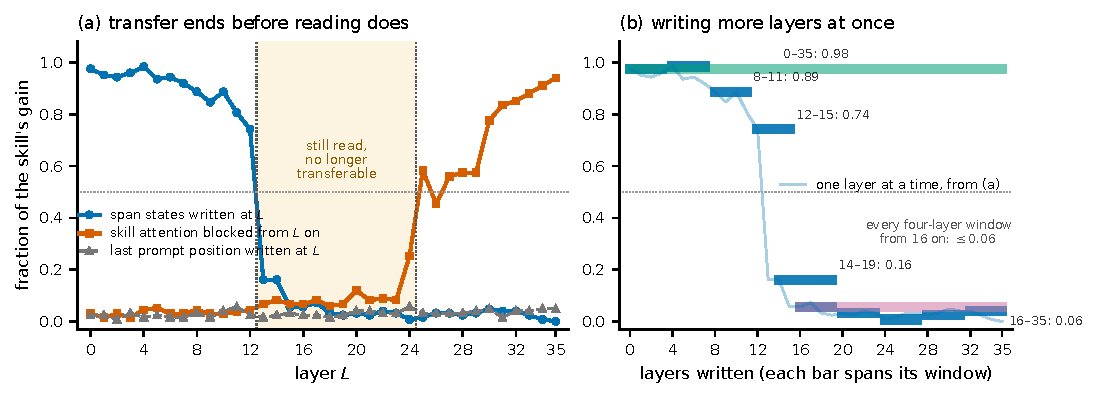
\includegraphics[width=\textwidth]{fig-transfer-reading.pdf}
\caption{Depth profiles for all eight main model--benchmark comparisons. Blue shows
skill-span transfer recovery $\rho(L)$ in a wrong-skill receiver.
Orange shows aggregate skill-attention dependence $d(L)=1-q(L)$: the fraction
of originally correct answers lost after cumulative attention knockout
in the correct-skill execution. Shading spans the first half-effect
boundaries, highlighting weak transfer despite strong dependence; later
recrossings remain visible. Boundary layers are marked above each panel.
Each panel uses common eligible item IDs for both curves, with each run's
own baselines and execution protocol; $G$ denotes skill groups. The
knockout affects both access from post-skill tokens and skill-state updates. Every plotted
layer is measured.}
\Description{Eight line plots show transfer recovery declining before skill-attention dependence subsides on their common eligible populations.}
\label{fig:transferreading}
\end{figure*}
